\chapter{Konzept und Systemdesign}
\printmyminitoc{1}

\section{Aufbau Schiffsysteme}
Wie werden die Motoren im Schiff angesteuert?
Welche Angriffsmöglichkeiten gibt es?
Wie wird das Ruder angesteuert?
Gibt es noch weitere wichtige Systeme?

\section{Steuerungslogik des Controllers}
Der benutzte Controller ist ein XBox Series X Controller. Dieser wurde gewählt, da er eine gute Haptik hat und 
viele Tasten besitzt. Zusätzlich ist er kabellos und kann somit frei bewegt werden. Um die Steuerung des Schiffes zu
ermöglichen, müssen die Eingabgen des Controllers in Steuerbefehle umgewandelt werden. Dies passiert auf dem 
Raspberry Pi. Der Controller wird über Bluetooth mit dem Raspberry Pi verbunden. Dort werden die Eingaben des Controllers
ausgelesen und in einem Python-Script in Steuerbefehle umgewandelt. \\
Um eine intuitive Steuerung zu ermöglichen, muss das Konzept des Controllers gut durchdacht sein.
Da der XBox Controller viele Tasten besitzt und die Steuerung des Schiffes nicht zu komplex sein soll,
werden einige Tasten nicht verwendet. 
\begin{figure}[H]
    \centering
    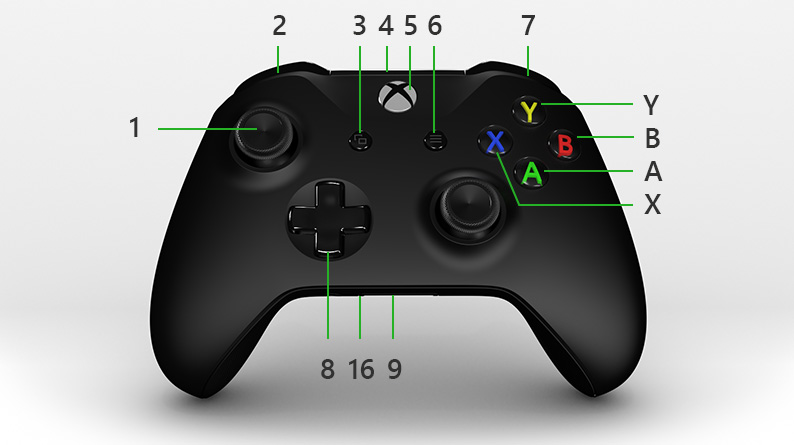
\includegraphics[scale=0.5]{images/vorderseite.jpg}
    \caption{Vorderseite des Controllers}
    \label{fig:vorderseite}
\end{figure}

\begin{figure}[H]
    \centering
    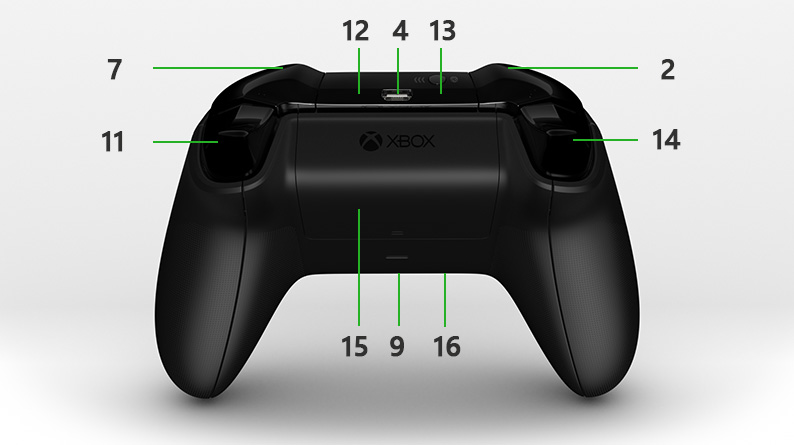
\includegraphics[scale=0.5]{images/rueckseite.jpg}
    \caption{Rückseite des Controllers}
    \label{fig:rueckseite}
\end{figure}

\begin{table}[H]
    \begin{tabular}{|c|c|}
    \hline
    \rowcolor[gray]{0.8}
     Nummerierung der Taste & Funktion \\ \hline 
     1& 1 \\ \hline 
     1& 1 \\ \hline 
    \end{tabular}
\end{table}

\section{Integration des Rogue Device}
Wie soll es mit dem Controller und dem Schiff verbunden sein?
\\
Was muss ich dabei beachten?
Muss eine Rückmeldung für die Eingaben geschehen? Wenn ja, wie?
(kleiner OLED-Bildschirm oder App)
